\documentclass[14pt]{extbook}
\usepackage{multicol, enumerate, enumitem, hyperref, color, soul, setspace, parskip, fancyhdr} %General Packages
\usepackage{amssymb, amsthm, amsmath, latexsym, units, mathtools} %Math Packages
\everymath{\displaystyle} %All math in Display Style
% Packages with additional options
\usepackage[headsep=0.5cm,headheight=12pt, left=1 in,right= 1 in,top= 1 in,bottom= 1 in]{geometry}
\usepackage[usenames,dvipsnames]{xcolor}
\usepackage{dashrule}  % Package to use the command below to create lines between items
\newcommand{\litem}[1]{\item#1\hspace*{-1cm}\rule{\textwidth}{0.4pt}}
\pagestyle{fancy}
\lhead{Module6}
\chead{}
\rhead{Version A}
\lfoot{2107-1615}
\cfoot{}
\rfoot{test}
\begin{document}

\begin{enumerate}
\litem{
Construct the lowest-degree polynomial given the zeros below. Then, choose the intervals that contain the coefficients of the polynomial in the form $x^3+bx^2+cx+d$.\[ 5 + 4 i \text{ and } -4 \]\begin{enumerate}[label=\Alph*.]
\item \( b \in [-2.3, 4.4], c \in [-1.6, -0.93], \text{ and } d \in [-21.5, -18] \)
\item \( b \in [-8.4, -5.6], c \in [0.11, 1.85], \text{ and } d \in [163.6, 167.2] \)
\item \( b \in [3, 9.5], c \in [0.11, 1.85], \text{ and } d \in [-165.4, -158.5] \)
\item \( b \in [-2.3, 4.4], c \in [-0.84, 0.88], \text{ and } d \in [-17.4, -12] \)
\item \( \text{None of the above.} \)

\end{enumerate} }
\litem{
Construct the lowest-degree polynomial given the zeros below. Then, choose the intervals that contain the coefficients of the polynomial in the form $ax^3+bx^2+cx+d$.\[ \frac{-1}{2}, \frac{-1}{4}, \text{ and } \frac{7}{5} \]\begin{enumerate}[label=\Alph*.]
\item \( a \in [35, 42], b \in [-88, -76], c \in [47, 56], \text{ and } d \in [-8, -2] \)
\item \( a \in [35, 42], b \in [-66, -63], c \in [4, 12], \text{ and } d \in [3, 13] \)
\item \( a \in [35, 42], b \in [20, 30], c \in [-38, -35], \text{ and } d \in [3, 13] \)
\item \( a \in [35, 42], b \in [-29, -24], c \in [-38, -35], \text{ and } d \in [3, 13] \)
\item \( a \in [35, 42], b \in [-29, -24], c \in [-38, -35], \text{ and } d \in [-8, -2] \)

\end{enumerate} }
\litem{
Describe the zero behavior of the zero $x = 8$ of the polynomial below.\[ f(x) = -7(x - 2)^{10}(x + 2)^{6}(x + 8)^{11}(x - 8)^{6} \]\begin{enumerate}[label=\Alph*.]
\begin{multicols}{2}\item 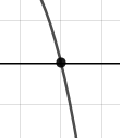
\includegraphics[width = 0.3\textwidth]{../Figures/polyZeroBehaviorAA.png}\item 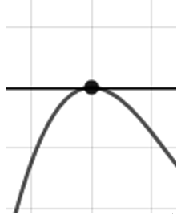
\includegraphics[width = 0.3\textwidth]{../Figures/polyZeroBehaviorBA.png}\item 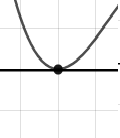
\includegraphics[width = 0.3\textwidth]{../Figures/polyZeroBehaviorCA.png}\item 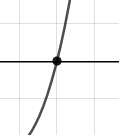
\includegraphics[width = 0.3\textwidth]{../Figures/polyZeroBehaviorDA.png}\end{multicols}\item None of the above.
\end{enumerate} }
\litem{
Describe the zero behavior of the zero $x = 8$ of the polynomial below.\[ f(x) = -9(x - 5)^{12}(x + 5)^{9}(x + 8)^{10}(x - 8)^{7} \]\begin{enumerate}[label=\Alph*.]
\begin{multicols}{2}\item 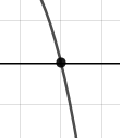
\includegraphics[width = 0.3\textwidth]{../Figures/polyZeroBehaviorCopyAA.png}\item 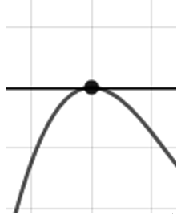
\includegraphics[width = 0.3\textwidth]{../Figures/polyZeroBehaviorCopyBA.png}\item 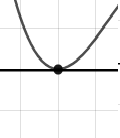
\includegraphics[width = 0.3\textwidth]{../Figures/polyZeroBehaviorCopyCA.png}\item 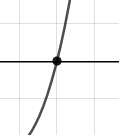
\includegraphics[width = 0.3\textwidth]{../Figures/polyZeroBehaviorCopyDA.png}\end{multicols}\item None of the above.
\end{enumerate} }
\litem{
Which of the following equations \textit{could} be of the graph presented below?
\begin{center}
    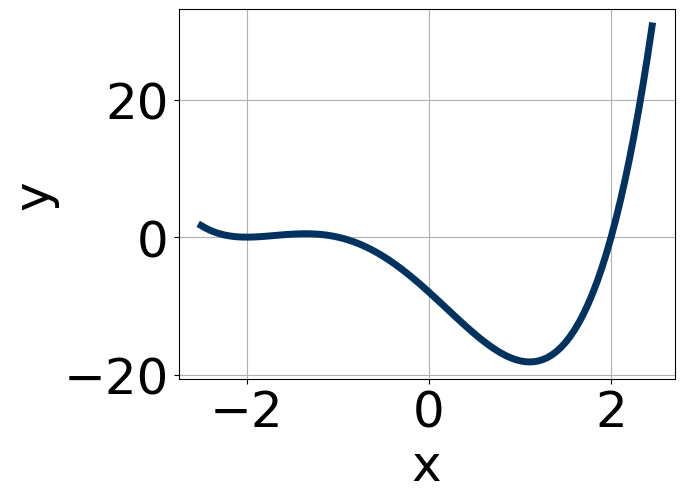
\includegraphics[width=0.5\textwidth]{../Figures/polyGraphToFunctionCopyA.png}
\end{center}
\begin{enumerate}[label=\Alph*.]
\item \( -8x^{7} (x + 4)^{4} (x + 1)^{11} \)
\item \( -14x^{10} (x + 4)^{8} (x + 1)^{9} \)
\item \( -17x^{4} (x + 4)^{4} (x + 1)^{6} \)
\item \( 14x^{10} (x + 4)^{6} (x + 1)^{9} \)
\item \( 13x^{8} (x + 4)^{10} (x + 1)^{10} \)

\end{enumerate} }
\litem{
Describe the end behavior of the polynomial below.\[ f(x) = 5(x + 3)^{3}(x - 3)^{8}(x + 7)^{3}(x - 7)^{5} \]\begin{enumerate}[label=\Alph*.]
\begin{multicols}{2}\item 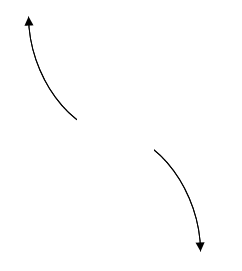
\includegraphics[width = 0.3\textwidth]{../Figures/polyEndBehaviorAA.png}\item 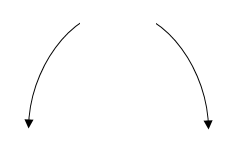
\includegraphics[width = 0.3\textwidth]{../Figures/polyEndBehaviorBA.png}\item 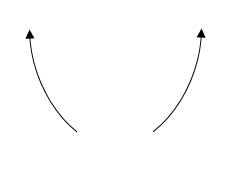
\includegraphics[width = 0.3\textwidth]{../Figures/polyEndBehaviorCA.png}\item 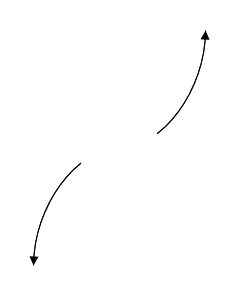
\includegraphics[width = 0.3\textwidth]{../Figures/polyEndBehaviorDA.png}\end{multicols}\item None of the above.
\end{enumerate} }
\litem{
Construct the lowest-degree polynomial given the zeros below. Then, choose the intervals that contain the coefficients of the polynomial in the form $x^3+bx^2+cx+d$.\[ -4 - 5 i \text{ and } 4 \]\begin{enumerate}[label=\Alph*.]
\item \( b \in [-8, -3], c \in [8.79, 9.4], \text{ and } d \in [160, 168] \)
\item \( b \in [-1, 2], c \in [0.48, 1.62], \text{ and } d \in [-24, -18] \)
\item \( b \in [2, 5], c \in [8.79, 9.4], \text{ and } d \in [-165, -163] \)
\item \( b \in [-1, 2], c \in [-0.13, 0.06], \text{ and } d \in [-18, -14] \)
\item \( \text{None of the above.} \)

\end{enumerate} }
\litem{
Construct the lowest-degree polynomial given the zeros below. Then, choose the intervals that contain the coefficients of the polynomial in the form $ax^3+bx^2+cx+d$.\[ -7, \frac{-3}{2}, \text{ and } \frac{-5}{3} \]\begin{enumerate}[label=\Alph*.]
\item \( a \in [0, 7], b \in [-44, -36], c \in [-26, -17], \text{ and } d \in [101, 112] \)
\item \( a \in [0, 7], b \in [59, 62], c \in [138, 153], \text{ and } d \in [-109, -103] \)
\item \( a \in [0, 7], b \in [59, 62], c \in [138, 153], \text{ and } d \in [101, 112] \)
\item \( a \in [0, 7], b \in [-26, -18], c \in [-119, -111], \text{ and } d \in [-109, -103] \)
\item \( a \in [0, 7], b \in [-65, -60], c \in [138, 153], \text{ and } d \in [-109, -103] \)

\end{enumerate} }
\litem{
Describe the end behavior of the polynomial below.\[ f(x) = -4(x - 5)^{3}(x + 5)^{4}(x + 6)^{3}(x - 6)^{3} \]\begin{enumerate}[label=\Alph*.]
\begin{multicols}{2}\item 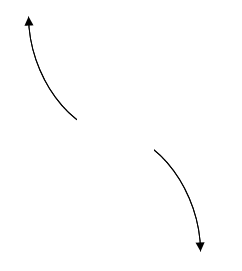
\includegraphics[width = 0.3\textwidth]{../Figures/polyEndBehaviorCopyAA.png}\item 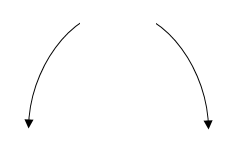
\includegraphics[width = 0.3\textwidth]{../Figures/polyEndBehaviorCopyBA.png}\item 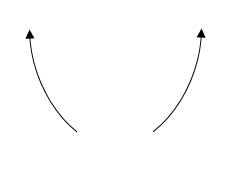
\includegraphics[width = 0.3\textwidth]{../Figures/polyEndBehaviorCopyCA.png}\item 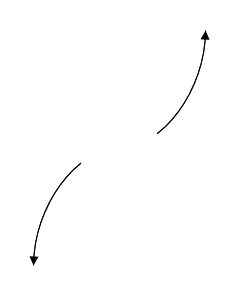
\includegraphics[width = 0.3\textwidth]{../Figures/polyEndBehaviorCopyDA.png}\end{multicols}\item None of the above.
\end{enumerate} }
\litem{
Which of the following equations \textit{could} be of the graph presented below?
\begin{center}
    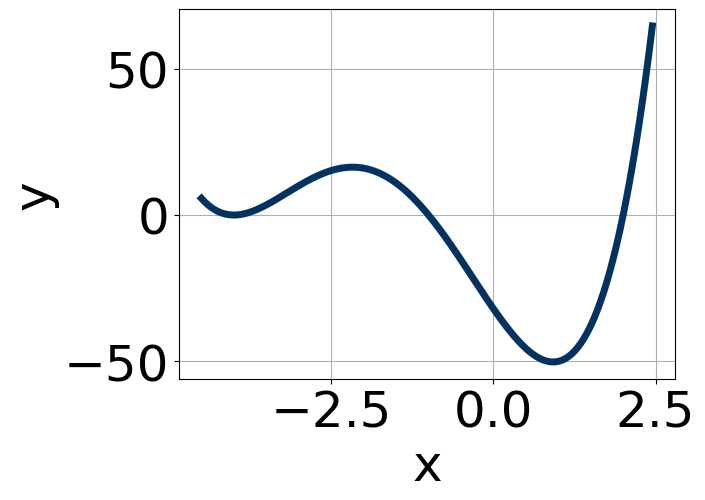
\includegraphics[width=0.5\textwidth]{../Figures/polyGraphToFunctionA.png}
\end{center}
\begin{enumerate}[label=\Alph*.]
\item \( 10x^{11} (x + 1)^{4} (x - 1)^{5} \)
\item \( -8x^{7} (x + 1)^{8} (x - 1)^{10} \)
\item \( -12x^{9} (x + 1)^{8} (x - 1)^{5} \)
\item \( 3x^{10} (x + 1)^{4} (x - 1)^{11} \)
\item \( -10x^{9} (x + 1)^{9} (x - 1)^{10} \)

\end{enumerate} }
\end{enumerate}

\end{document}